\begin{figure*}[t]
\centering
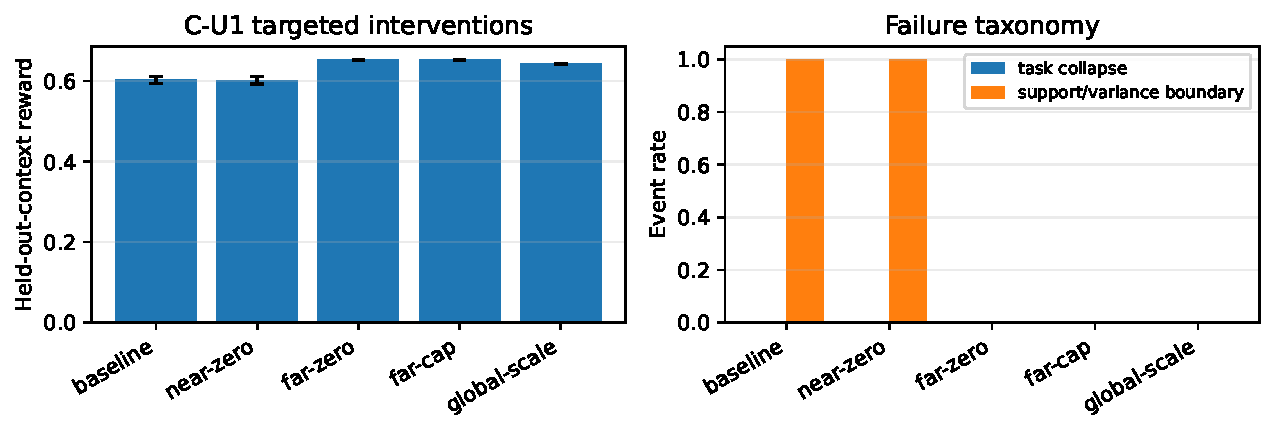
\includegraphics[width=0.93\textwidth]{figures/generated/fig3_cu1_causal.pdf}
\caption{C-U1 causal intervention with learnable variance. The left panel reports registered held-out-context reward with confidence intervals; the right panel separates task-performance collapse from support or variance-boundary events. Near-zero tracks the uncontrolled baseline, while Far-zero and Far-cap remove the task-collapse pathway without introducing NaN/Inf failures.}
\label{fig:cu1-causal}
\end{figure*}
\begin{table}[t]
\centering\small
\caption{C-U1 intervention summary (20 seeds).}
\label{tab:cu1-causal}
\begin{tabular}{lccc}
\toprule Method & Reward & Task event & Boundary event \\
\midrule
baseline & 0.603 & 0.00 & 1.00 \\
near-zero & 0.602 & 0.00 & 1.00 \\
far-zero & 0.653 & 0.00 & 0.00 \\
far-cap & 0.653 & 0.00 & 0.00 \\
global-scale & 0.643 & 0.00 & 0.00 \\
\bottomrule
\end{tabular}
\end{table}
